\chapter{Language and What I mean Language}

\begin{quotation}
  The fundamental aim in the linguistic analysis of a language L is to separate the grammatical sequences which are the sentences of L from the ungrammatical sequences which are not sentences of L. 
  The grammar of L will thus be a device that generates all of the grammatical sequences of L and none of the ungrammatical ones. \\

  Noam Chomsky - Syntactic Structures (2nd Edition) de Gruyter Mouton (2002)
\end{quotation}

因为我只是一个业余的爱好者, 所以对于计算机语言的思考本该不是我所能够发言的, 我只能做到一个将前人的思想和智慧做一个整理和转述而已. 并且我的理解不一定正确, 请见谅. \footnote{假如你觉得不够过瘾的话, 可以看看我的参考资料, 或者你觉得我在哪里有所不足的话, 欢迎指出. }

\section{Magic is Basic \footnote{我记得阿瑟克拉克曾经说过, 一切科技发展到了一定程度都会像是魔法一样. 这样的原因究竟是因为科技发展得太过高级和复杂呢? 还是因为科技的使用的过程中存在着抽象的构造, 导致了人们不需要了解科技内部的构造和原理, 所以导致了使用过程中的无意识呢? 我说不清楚. \\ 虽然抽象的方式可以使用简单的原理构造出复杂的过程, 也可以将复杂的过程抽象为简单的过程, 这样让使用者可以轻松地使用, 也会导致使用者可能会盲目地使用, 最终失去了对技术的理解而变成了像是面对魔法一样的敬畏和恐惧. \\ 但是我认为, 哪怕是魔法, 也是有吟唱的技术的, 出了错的话就会爆炸之类的. 所以我们完全没必要神话技术, 只需要找到技术背后的计算过程的一些简单的原理, 我们就能够理解并实现最后的咒术吟唱. 然后成为大魔法师. 所以魔法是很简单的, 科技也是如此, 其实是一种每个人都能掌握的技术. }}
\begin{quotation}
  心智的活动, 除了尽力产生各种简单的认识之外, 主要表现在如下三个方面: \\
  1) 将若干简单认识组合为一个复合认识, 由此产生出各种复杂的认识. \\
  2) 将两个认识放在一超对照. 不管它们如何简单或者复杂. 在这样做时并不将它们合而为一. 由此得到有关它们的相互关系的认识. \\
  3) 将有关认识与那些在实际中和它们同在的所有其他认识隔离开. 这就是抽象. 所有具有普遍性的认识都是这样得到的. \\

  John Locke - An Essay Concerning Himan Understanding (1690)\footnote{来自SICP. 一本我觉得很好的书. }
\end{quotation}

\subsection{Intro: Once upon a Time}
回忆小学学习算术的过程: 老师亲切地站在讲台上, 告诉下面的一帮小屁孩, 同学们, 你们看, $1 + 2$ 就是把 $1$ 加上 $2$, 然后就是 $3$. \footnote{具体的到底有没有说是一个手指加上两个手指就是$3$, 还是一个苹果加上两个苹果就是三个苹果什么的, 我已经完全记不得了. 但是这个时候假如有个天赋异禀的小孩子说了一句, 老师, 我还知道$2+1=1+2$因为这个关于加法组成一个Abel交换群. 害, 一个法国数学笑话了. }我们就不解释这个加法的过程了, (很遗憾, 我也不得不默认你们知道一些东西, 像那些一般的教材一样为了简洁而略去许多的说明), 如果只是形式地看看这个算式的话: \footnote{下面的例子来源于王垠的\href{http://www.yinwang.org/blog-cn/2018/04/13/computer-science}{博客}, 里面的东西比我的要多, 并且我觉得写得比较有意思. }

$$ 1 + 2 $$

我们会发现, 这个算式有着这样的结构: 符号$+$将它左边的东西, 不管是什么, 和右边的东西加在一起, 然后得到了一个值(在这里就是$3$). 

然后, 我们会接触到更加复杂的数学表达式, 比如: 

$$1 + 2 \times (3 + 4 / 2)$$

这个公式计算肯定是不太麻烦的, 但是如果我们不在乎这个公式到底在做什么, 而是形式上的思考这个公式的形式结构, (为了减少计算符号的优先级, 我们可以将这个公式加上括号来看): 

$$1 + (2 \times (3 + (4 / 2)))$$

虽然这个公式非常的简单, 估计大多数的人都能一眼望穿, 但是请想想当年那个还在抠鼻屎玩的那个小屁孩, 小孩子接触到这个算式的时候是如何计算的? 大概是这样的一个过程: 

首先看到的是最外层的这个加号, 然后就要将$1$和括号的值加起来, 于是去计算括号, 也就是$2 \times (3 + (4 / 2))$的值, 然后就要将$2$和新的括号$(3 + (4 / 2))$的值乘起来, 于是为了计算$3 + (4 / 2)$的值, 继续往括号里面看... 如此往复, 直到到了最后一层的括号里面, 因为没有更深的括号了, 所以就只是一个简单的表达式, 可以进行简单的计算了. \footnote{这里我最近有一个想法, 就是是不是可以理解为我在看到优先级更高的计算的时候, 我将目前在做的事情先搁在一边, 类似于保存一个状态, 等到优先级更高的计算完成之后, 再回到原来的状态, 和新的结果进行一个运算, 相当于是推迟了计算. 有一个延时的感觉. }

于是我们计算出了最终的$4 / 2$的值$2$, 然后将这个值代回上一层的括号里面, 计算出$3 + 2$的值$5$, 然后计算$2 \times 5$的值$10$, 然后再计算$1 + 10$的值... \\

天呐, 原来口算竟然是这么复杂的一件事情吗? 看来我口算水平差也是情有可原了. 当然不是, 我们会发现, 第一步的过程, 也就是"看"表达式的过程, 在我们的大脑里面几乎是潜意识一般自动地处理的, 而第二步的算值的过程, 则不过是非常简单的两个数之间的四则运算而已. \footnote{相比对于四则运算你应该是没什么问题的了, 所以我们就将第二步的分析给略了先. }

在第一步的时候, 我们并不关心表达式的值, 而是关心表达式的形式结构, 然后在解构了表达式的形式结构之后, 我们得到了表达式的一个类似于下面的图形一样的逻辑结构: 

\begin{figure}[h]
  \centering
  \begin{tikzpicture}
    \tikzset{grow'=right,level distance=60pt}
    \tikzset{execute at begin node=\strut}
    \tikzset{every tree node/.style={anchor=base west}}
    \Tree [.Add [.Mutiply [.Add [.Divide [.4 ] [.2 ]] [.3 ]] [.2 ] ] [.1 ]]
  \end{tikzpicture}
  \caption{一个简单的图示}
\end{figure}

下面的例子虽然看起来非常"可怕"\footnote{其实不过就是一个极限的定义, 是从我的教科书上抄来的, 为了方便讲解}, 但是我们只会从形式上去看看这个东西, 所以不要害怕. 因为你会发现除了简单的加法, 一些复杂抽象的数学符号也是同样拥有着类似的形式结构(因为排版的缘故, 所以图跑了, 但是没关系, 翻到下一页就能够见到了. ): 

$$\forall \varepsilon > 0 (\exists N \in \mathbb{N} (\forall n > N \in \mathbb{N} (\vert a_n - a \vert < \varepsilon)))$$

\begin{figure}[h]
  \centering
  \begin{tikzpicture}
    \tikzset{grow'=right,level distance=60pt}
    \tikzset{execute at begin node=\strut}
    \tikzset{every tree node/.style={anchor=base west}}
    \Tree [.Forall [.Epsilon [.Greater [.Epsilon ] [.0 ]]] [.Exists [.N [.In [.Natural\ Number ]]] [.Forall [.n [.Greater [.n ] [.N ]]] [.Abs [.Sub [.an ] [.a ]] [.Epsilon ]]]]]
  \end{tikzpicture}
  \caption{还是一个简单的图示}
\end{figure}

这个东西虽然看起来好像是那么一回事, 但是在形式的分解下, 就会变成一堆非常简单的小关系, 或者是小逻辑, 小运算. 这样的分解就让我们能够理解和处理庞大的东西或者是抽象的东西. 

其实我认为不仅是学习算术的过程, 比如我们在日常表达的过程中, 或者是读一句话的时候, 我们也有类似的解析过程. 比如说下面这句话: 

\begin{quote}
  幸せな君の隣にいたいよ
\end{quote}

我们可以将这个句子分解成下面的结构\footnote{首先声明一下, 我不会日语, 我也不会什么语法分析, 也许以后会学, 但是现在不会, 这个可能只能算是我的一种瞎掰而已, 不过无伤大雅, 可以使用就好. }: \emph{((((幸せな)君)の)隣に)いたいよ}, 变成这样的结构之后, 每一个部分都不过是一个(看起来)简单的东西了. \footnote{然后在理解的时候, (有点像是上面的求值计算过程), 就会变成这样: ((((幸福的)你)的)身边)待着. 假如再加入一点点"达"的成分, 没准可以翻译成待在幸福的你的身边. 不过这个应该没关系了. 假如你觉得上面的例子有点不太过瘾, 你没准可以将这个模型应用到其他的语言里面, 虽然我不能保证一定适用但是我能够保证这个一定适用, 但是总归是一个有意思的思考方式. 并且我认为我的英语就是这么一个理解的过程的. 嗯, 加入以后有可能的话, 感觉可以试试往这个方向上做一些东西. }

那么这和计算机语言又有什么关系呢? 抖个机灵, 没关系, 因为世界上不存在所谓的计算机语言: 

\begin{quotation}
  My conscience won't let me call Ruby a \emph{computer} language. That would imply that the language works primarily on the computer's terms. That the language is designed to accommodate the computer, first and foremost. That therefore, we, the coders, are foreigners, seeking citizenship in the computer's locale. It's the computer's language and we are translators for the world. \\
  But what do you call the language when your brain begins to think in that language? When you start to use the language's own words and colloquialisms to express yourself. Say, the computer can't do that. How can it be the computer's language? It is ours, we speak it natively!\\
  We can no longer truthfully call it a \emph{computer} language. It is \emph{coderspeak}. It is the language of our thoughts.\\

  why the lucky stuff - \href{https://poignant.guide/book/chapter-3.html}{Why's (poignant) Guide to Ruby}
\end{quotation}

当然, 相比自然语言, 计算机语言为了方便计算机的理解, 它的结构形式就非常的明显并且简单, 比如经常被自己的圆括号表达形式而被嘲讽的Lisp语言, \footnote{有一个非常不恰当的比喻, 就是Lisp就像是中国的社会主义的思想是非常的美妙, 但是其他某些人说, 诶, 你好无聊啊, 有那么多括号, 你的形式好奇怪啊. 然后就被边缘化了. 然而很多语言都在"暗地"里学习Lisp的特性, 比如宏(marco), Lambda演算, eval等等. 因为感觉是真的香. }或者是形式比较单一呆板的汇编语言, \footnote{呃, 这个暂时不要求. 因为我认为学习汇编对理解计算机程序设计没有帮助. 但对理解计算机构造比较有用. 还是先学设计, 对文科生友好一点... }虽然它们的的形式结构虽然在某种程度上面给人一种不明觉厉的高级感, 但是假如你不要把它们想得那么复杂可怕, 其实编程语言就是这样的一个东西: 一种有着特定形式的语句, 按照这些语句所表现的一种结构能够用来描述逻辑过程. 就像是普通的汉语或者英语一样, 是用来描述或者表达一种过程的. 

本来到了这里我应该至少开始介绍一门编程语言了, 然后让你在计算机屏幕上面打印个什么, Hello World, 是吧? 然后让你乐乐, 觉得自己很厉害, 然后被我骗进来学一堆乱七八糟的东西, 最终成为掉头发的社畜. 呃, 我说了, 我只是一个业余爱好者, 并且我发现前面的风格如此随意, 就不太好突然降智, 画风突转什么的, 所以我打算把语言的介绍再往后推一点点. 就一点点. \footnote{可以去读一下why的书的第三章, 我最近会把它翻译掉. }

回到之前的小学算术题目: $(1 + (2 \times (3 + (4 / 2))))$, 假如我们已经分解好了结构, 那么每一次的计算只不过是加减乘除的最简单的操作了. 

计算机其实也就是这样的, 它能够做到的也就只有简单的计数和运算而已, 之所以能够实现那些像魔法一般的神奇的结果, 其背后也不过就是最简单的运算而已. 计算机在处理编程语言的时候会将它们分解成一定的结构, 然后再对那些最小的结构进行运算和处理. 

举一个例子: 

$$\sum_{i = 1}^5 i$$

假如我们不是伟大的高斯同学, 看到了这个$\sum$符号, 我们可能会把它看作是这样的东西: 对于每一个$i$从$1$到$5$, 将它们都加在一起. 对于人来说, 这很轻松: $1 + 2 + 3 + 4 + 5$, 虽然麻烦了一点. \footnote{传说是高斯同学在小学的时候发明了对这样的级数的求和公式. 但是我们不会这样来做. }

那么按照前面朴素的想法, 肯定会想要知道这个结构是什么样的呢? 没错, 就是: $(1 + (2 + (3 + (4 + (5)))))$. 假如我们是一个不那么聪明的计算机, 我们会这样做: 将$4 + 5$的结果和$3$相加, 然后将这个结果再和$2$相加... 虽然这个过程用语言来描述会又臭又长. 但是假如你写了很多的话, 就会发现好像这个过程有一定的规律: 将 什么 和 什么 相加, 这个相加的结果重新用来进行新的一轮的加法. 用语言来描述太复杂了, 用数学来表示: 

$$ sum(i) = sum(i - 1) + i , sum(1) = 1$$

这样的写法是不是比较抽象? 那么要不我们把它们替换看看? 

\begin{figure}[h]
  \centering
  \begin{tikzpicture}
    \tikzset{grow'=right,level distance=60pt}
    \tikzset{execute at begin node=\strut}
    \tikzset{every tree node/.style={anchor=base west}}
    \Tree [.sum(5) [.sum(4) [.sum(3) [.sum(2) [.1 ] [.2 ]] [.3 ]] [.4 ] ] [.5 ]]
  \end{tikzpicture}
  \caption{还是一个简单的图示}
\end{figure}

这样的展开的形式是不是就能够理解了? 每一次做的事情是不是就不过是加法而已? 并且假如你想要计算$\sum_{i = 1}^5 f(i)$的话, 是不是只需要将上面的数学公式描述改为$ sum(i) = sum(i - 1) + f(i) , sum(1) = f(1)$即可了? 假如你想要计算$\sum_{i = 1}^5000 f(i)$, 那么也非常轻松, 结果不就是$sum(5000)$嘛. 什么? 你问我结果是什么? 至少我是不会真的用手去算的. 我只会告诉你, $sum(5000)$就是一个这样的过程得到的结果: 这样的结果是将$f(i)$从$1$到$5000$的取值相加的过程的结果. \footnote{这里我觉得有必要来一点点的代码了: \mintinline{ruby}{def sum(i, f); i == 1 ? 1 : sum(i - 1, f) + f.call(i); end}. 之所以写成行的形式是因为我不知道怎么在注释里面写换行的代码. 但是我还是不开始讲编程语言, 诶, 就是玩. }

上面的过程里面, 我们做的事情就是将一个求和的过程来分解成一组计算机能够理解的简单过程. 这样的话, 我们就可以让计算机来为我们干活了. 不过可惜的是, 我们的数学语言和自然语言可能很难对计算机生效. 所以学习一点点的计算机语言有点必要了. 

\subsection{异乡人啊, 你的管风琴在唱着什么歌谣呢? }
\begin{quotation}
一日一夜に 月は照らずとも

悲傷しみに 鵺鳥鳴く

吾がかへり见すれど 花は散りぬべし

慰むる心は 消ぬるがごとく

新世に神集ひて 夜は明け鵺鳥鳴く

咲く花は 神に祈ひ禱む

生ける世に 我が身悲しも

夢は消ぬ 怨恨みて散る
\\
\emph{傀儡謠─怨恨みて散る} \footnote{来自我很喜欢的电影里面的音乐. \href{https://music.apple.com/cn/album/kugutsu-uta-uramite-chiru/1547968823}{Apple Music: Kugutsu Uta Uramite Chiru}. \\电影里面的故事比较有意思, 当虚假和现实难以区分的时候, 那么我们该对虚拟保持什么态度? 计算机技术其实已经发展到了能够实现电影里面哲思的地步了: 比如押井守(导演, 或者叫监督? )就认为手机就像是影片中的电子脑 -- 影片中的世界, 人们无法离开资讯世界与电子脑, 现实生活中, 人们也同样无法离开手机或者电脑, 或者说, 由它们组成的资讯的世界. 人与人之间的连接越来越多(lain), 但是连接的关系越来越脆弱... 就像是蜘蛛结网, 为了在摇曳的风中保持着网的完好, 不得不向四面八方射出自己的丝, 肚囊因此越来越扁. \\虚拟的困境在于其是转瞬即逝的. 这个无关技术是否先进. 我还记得蒋勋说红楼梦里面有一段故事, (大意) 讲的是一个大户人家, 千金小姐嫁人, 华贵的轿子在路上遇雨, 躲到和另一户贫穷人家的小轿子遇见了, 处于同情心, 她就将自己妈妈送给她的一个陪嫁品 -- 一个小小的像首饰盒一样的东西送给了那位穷小姐. 毕竟那个盒子看起来也十分不起眼. 然而命运多舛, 她嫁的家庭一瞬间荣华富贵全部消失, 自己也沦落一个普通的打杂的人, 在一家大户人家打工. 这家大户人家的主人有一间珍贵的阁楼, 不让任何人进去, 有一次这位曾经的千金小姐机缘巧合地走进了那间阁楼, 却突然发现里面供奉着的就是自己当初送给那位穷小姐的首饰盒 -- 原来那位穷小姐一家靠首饰盒里的财富做生意才发了家. 荣华富贵就是这样一瞬间来, 一瞬间去, 好像一切都是那么虚幻和飘渺, 转眼之间一切都改变了. \\啊, 好像有点偏离我们书本的内容了. }
\end{quotation}

这是一首日语的歌曲的歌词. 我摊牌了, 其实我不会日语, 所以下面的所有关于日语的语法的说法, 绝对是我的一己之见, 请学日语专业的同学饶过我. 但是没见过猪跑, 总是吃过猪肉的. 看到这么一串奇怪的东西, 你的眼睛(大概)肯定会想要去寻找你熟悉的汉字. 然后在这个过程中, 虽然这些汉字怪怪的, 但是你估计会下意识地将它们转换为简体字, 然后再尝试处理它们的意思. \footnote{这也是为什么我选择日语的原因, 因为它们借鉴了很多的中文, 假如直接放汉字的话, 就太容易识别了. 无法体现出我接下来讲的语法处理的过程. 又, 还有一个原因是因为日语和中文一样, 好像都是属于图形字符, 这也是为什么弹幕视频网站在中国和日本比较流行, 而在欧美国家很少. 因为英语之类的东西很难像汉字一样模糊地阅读. } 比如在"新世に神集ひて 夜は明け鵺鳥鳴く"一行里面, 我们可以先将那些词语进行一个替换(以及断句和联想): "新 世(界) * 神 (聚)集 * *  夜(晚) * 明(亮) * 鵺鸟\footnote{有说是一种妖怪, 也有说是一种画眉鸟的, 这我就没法说了. \href{https://zh.wikipedia.org/wiki/鵺}{维基百科}} 鸣(叫)". 

假如说我告诉你, 在日语里面的很多的语法结构有像这样的形式: 修饰 + 对象 + 动作. \footnote{注意, 这个语法说法是我杜撰出来的. 科不科学我不知道, 但是秉承着物理的不完全归纳法, 猜的厚脸皮我还是有的. \\ 其实之所以这样讲, 也是为了用来引出之后Ruby的语法: \mintinline{ruby}{UI::Button.new()}, 如果你会的话, 估计会觉得比较像. 没错, 就是因为我故意选的例子的原因. 这也是为什么你觉得很多教科书上的例题都很好, 然后实际拿来计算的时候就觉得不太对劲的原因之一吧. } 那么我们再用之前的结构的形式来给上面的那句话一个结构: (((新)(世界))(神)(聚集)), (((夜)(明))(鵺鸟)(鸣叫)). 这样的话, 根据结构代入那些小单元, 解释含义就能够得到语句的意思: (大概翻译) 新世界的神聚集, 夜明(黎明)时鵺鸟鸣叫. 
% \footnote{这样的解释我们不妨用Ruby的语法来进行一个比对: \mintinline{ruby}{新世界::神.聚集; 夜明::鵺鸟.鸣叫}, 这里我将\textbf{新世界}和\textbf{夜明}当作了一个命名空间, 然后\textbf{聚集}和\textbf{鸣叫}看成了类方法. 感觉写成\mintinline{ruby}{新世界::神.new.聚集; 夜明::鵺鸟.new.鸣叫}会更好一点. 不过其实都不是特别好就是了, 牵强附会的话总是有点困难, 还是再等等铺垫一个更好的出场机会吧. }

假如没有前面的一个分析过程, 直接遇到这样一个陌生的语言的文本, 哪怕是其中好像有一些熟悉的字眼, 可能也难以理解文本的意思吧. 那么思考里面的过程, 因为有了结构将语句分解成了简单的单元, 于是只需要理解简单的单元的含义, 就能够(通过结构)知道复杂语句的内容了. 并且这个时候文本中的熟悉的字眼就成为了辅助我们理解语句的工具了. 

其实对于一开始学习计算机语言的话, 我们还是先从形式上来理解语言, 这样的话, 我们就能够阅读. 这里建议阅读附录中对Why's (Poignant) Guide to Ruby中的部分翻译文字, 我会从别的角度来介绍形式. \footnote{之后我们会接触各种各样的语言, 也就会接触各种各样的形式. 不过和自然语言相比, 计算机语言因为是一种类似于人造的语言, 所以相比有着更多形式的, 更多语法的自然语言, 计算机语言的形式其实都是非常简单的. }

% 比如说: \footnote{下面的代码我不建议运行, 因为这些是我按照Ruby的形式和语法瞎写的乱七八糟的东西, 谁知道会不会出问题. 并且也不建议记住, 更不建议去背或者去死记具体函数的用法. 只要关注这个语言的形式. 并且联系我们之前对那段日语歌词的做法, 因为下一节才是真正开始教你一点点Ruby的时候, 现在还请忍耐一下, 关注其中的语言形式吧. }

Peter Norvig在其书PAIP中写道: "Learning a language involves remembering vocabulary items (or knowing where to look them up) as well as learning the basic rules for forming expressions and determining what they mean. " 在我读到这段话后, 我就决定按照这样的方法来展开我的书本. \footnote{其实why的书的做法就是这样的. }即, 我们先仅仅从形式的角度来观察语言. 而不必理解其中的太多的原理和含义. 

毕竟每一个方士做法的时候, 都要搭起法台, 做好仪式的形式工作. 并且形式的摆放有时候也能够产生巨大的作用. \footnote{"谓东方青帝灵威仰, 主春生. 南方赤帝赤熛怒, 主夏长. 西方白帝白招拒, 主秋成. 北方黑帝汁光纪, 主冬藏, 中央黄帝含枢纽, 则寄王四时. 以四时化育, 亦须土也. 更加昊天上帝耀魄宝, 则为六帝. " 摘自\emph{吕思勉《理学纲要》第二篇}} 那么没关系, 为了进入这个魔法世界, 所以我们还是先从形式上入手, 至少搭好一个作法的平台, 能够读懂前辈道士用魔法咒术的形式传来的Wi-Fi密码... 

\begin{quotation}
  \begin{minted}{ruby}
    (3 - 2) * (3 + 2)
    1 ** 3
    5 / 3
    5.0 / 3
  \end{minted}
\end{quotation}

这些数学运算大概是比较简单的吧? 加(+)减(-)乘(*)除(/)还有乘幂(**), 都是一些比较熟悉的操作, 并且和数学里面的运算优先级一样, 都是从左到右, 括号优先, 乘幂最大, 其次乘除, 最后加减. \footnote{唯一需要注意的是, Ruby在处理整数(Integer)的除法的时候, 会和C一样保留整数, 也就是说, \mintinline{ruby}{5 / 3} 会得到1, 而对于浮点数(Float, 或者可以理解为带小数位的数)参与的除法, 如\mintinline{ruby}{5.0 / 3}, 则会得到1.66666667类似这样的结果. 不过这些不是我们目前需要着急在意的事情, 这些只是出于设计考量而做的一些妥协而已. 是一种类似于约定主义的东西. 请把目光聚焦在这些表达式的形式上吧. }

倘若我们想要把数学运算的结果保留下来, 那么我们可能在计算器(以卡西欧fx-991CN X为例)上这样操作: \fbox{1} \fbox{+} \fbox{1} \fbox{STO} \fbox{x}, 于是我们就能够把$1 + 1$的计算结果储存到变量$x$中了. 那么在Ruby里面, 我们可以这样形式地记做: 

\begin{quotation}
  \begin{minted}{ruby}
    x = 1 + 1
    money = 100 * x
    lunch_fee = 50
    money = money - lunch_fee
  \end{minted}
\end{quotation}

并且就像是数学里面对变量的计算一样, 我们可以像这样用变量来计算. 不过是一个形式而已. 于是看到类似的结构之后, 我们不妨就理解为x is 1 + 1. 

\begin{quotation}
  \begin{minted}{ruby}
    door = Door.new
    door.paint :red
    door.open
  \end{minted}
\end{quotation}

假如你会一点点英文的话, 上面那段文字估计就算不需要学计算机也是会的吧. \footnote{这个时候就可能会有人说, 啊, 少来了, 不过就是什么现在我们已经学会了1 + 1, 然后开始积分求和求累乘吧之类的. 呃, 怎么说呢, 还真是. 因为我觉得Ruby的很多美妙的操作是编程的程序员在相互维持着的, 比如那些很好看的method名字和很标准的ri文档, 这些虽然有Ruby本身的一些工具或者属性的夹持, 但是更多时候还是有赖于开发者的自觉. 比如要求良好的命名规范, 良好的注释, 以及duck philosophy(If something quarks like a duck, then treat it as a duck. )等等. 不过在自己写代码的时候可就不一定能够保证自己能够写出这样高质量的代码了, 所以假如你不注意的话, 就会写出一些看起来非常"极客"的东西: \mintinline{ruby}{var_0xfff.f_0x999.f_0x233 :aaza}. 假如还没有很好的排版(缩进)和注释, 就会导致整体的混乱以及难看. 不过嘛, 我们又不是什么自虐狂, 何必要这样折磨自己呢? 一般我们还是希望除了写代码的基本逻辑以外, 花一些时间和精力在美化代码, 或者让代码变得更加优雅之类的还是非常重要的. (虽然我觉得自己目前还没有那种能力... )\\不过也有因为这样导致的诟病, 比如说, 虽然和python很像, 但是python以其简洁和标准常常带来的是唯一的问题解决方案, 而Ruby却是写完了功能之后程序员为了追求奇技淫巧还在一直重构... 嘛, 没有什么好坏之分啦. }翻译翻译就是: door is a kind of Door. paint red to door. open the door. \footnote{虽然我突然发现日语的语序和这个真的是超级像诶: doorを赤く塗る, doorを開ける. }(door是一扇Door(门), door涂成了红色, door打开\footnote{这里我们就不要考虑什么主动型还是被动型了, 这点语法小问题而已, 宽容一点啦. })

这个时候我们相当于接触到了第一个在平时比较陌生, 但是在Ruby程序编程中的比较普遍存在的一种语言形式: \mintinline{ruby}{a.b(c)}. 这种形式在某种程度上可以说是Ruby的一个非常普遍存在的形式: 

\begin{quotation}
  \begin{minted}{ruby}
    player.move(:up, 1 * cm)
    player.attack :excalibur, enemy
    player.defence
  \end{minted}
\end{quotation}

上面那段有点像是一个RPG游戏了, player(玩家)在地图上向上走了1cm(厘米), player使用了excalibur(EX-咖喱棒)攻击enemy(敌人), player防御. 

如果仔细观察的话, 会发现这里的一些操作和上面的门的语句有一些十分类似的地方: 都是 \textbf{什么东西.做了什么动作(描述动作的一些信息)}, 或者是把括号去掉的形式. \footnote{这是因为Ruby比较灵活, 可以在它能够理解的范围内自动添加上括号. 但是假如会出现歧义的语句的时候, 就不能够这样忽略括号了, 否则会导致Ruby无法理解你想要表达的意思, 最后出错. }假如用一些专业一些的语言来说的话就是, 上面的语句的结构就是\textbf{对象.方法(方法参数)}. \footnote{英文的说法是\textbf{object.method(arguments)}, 其中方法的参数不一定只有一个, 并且也不一定只有特定的长度. }上面的"对象", "方法", "方法参数"我们不妨先采用形式化的定义而不是深究其具体的实现和原理. % 因为现在我们不要求理解这些的具体含义, 只要知道这样的形式以及其对应的一个名称, 以后解释的时候就会方便一点. 

有些时候, 虽然有时候会遇到某些看起来不像是满足上面的形式的代码, 这些代码其实是因为Ruby支持简化书写一小部分语法格式. \footnote{不知道这算不算是一种语法糖} 比如: 

\begin{quotation}
  \begin{minted}{ruby}
    print("I'm Groot. ")
    gets()
  \end{minted}
\end{quotation}

上面两个虽然看起来没有\mintinline{ruby}{a.b(c)}的形式, 但是假如将其完全书写, 就会发现其形式仍然是满足的. \\即 \mintinline{ruby}{Kernel.print("I'm Groot. ")}以及\mintinline{ruby}{Kernel.gets()}\footnote{Kernel是内核的一个意思. }的形式. 

我们传入的方法参数的形式有时候可以是空空如也的, 有时候可以是一连串的值, 有时候也可以是一些特殊的形式: 

\begin{quotation}
  \begin{minted}{ruby}
    5.times { print "I'm Lucky!!! " }
  \end{minted}
\end{quotation}

这句话有点像是: do the action of printing "I'm Lucky!!! " 5 times. (打印五次"I'm Lucky!!! ", 嗯, 人类的本质就是复读机. )

或者是: 

\begin{quotation}
  \begin{minted}{ruby}
    "I'm Lucky".each_char do |c|
      print c.upcase
    end
  \end{minted}
\end{quotation}

这句话就像是: do the action of printing the upper case of c, aka. each single character in the string "I'm Lucky". (取出"I'm Lucky"这串文字里面的每个字符, 简记为c, 将每个字符都以大写的方式打印到屏幕上去. )

也许你会觉得, 啊, 好麻烦啊, 上面两个例子又出现了一些新的形式, 这些形式好怪啊, 要学的东西好多啊. 还请不要怕, 其实我们并没有引入任何新的形式. 

其实在上面的代码中, 前半段的形式相比一定是让人十分眼熟的吧: \mintinline{ruby}{5.times}, \mintinline{ruby}{"I'm Lucky".each_char}就像是一种\mintinline{ruby}{a.b}的形式. 而后半段, 则出现了一个\textbf{do ... end}和\textbf{\{ ... \}}的形式. 这个时候, 我们不妨在形式上抽象地将其视为是一个整体, 就好像两者是一个特殊的"括号", "括号"里面包含了许多的内容. 这些内容具体是什么我们不必担心, 我们只需要像是对待字符串(一个被引号括起来的东西)一样, 对待这样的东西就好. 形式化地命名为代码块(block).

% 首先我们从至少还算是比较眼熟的部分开始看吧: \mintinline{ruby}{5.times}, \mintinline{ruby}{"I'm Lucky".each_char}其实和原来的object.method(arg)的形式是差不多的. 那么它们后面跟着的那一大块是什么? 假如我们不在意这个东西是什么的话, 但从形式上来看, 其实就是一个用\textbf{do ... end}包裹起来的一个东西, 里面好像填写了一些东西. 因为这样的结构比较独特, 并且有一定的意义, 我们以后就叫它代码块(block). 假如我们用一个名字(比如block)来替代这样的do ... end的组合块的话, 我们就会惊奇地发现, 其实这个的形式和我们之前看到的几乎是如出一辙的 -- \textbf{5.times block}. 是不是就像是把我们的代码块像参数一样传递给方法一样呢? 

所以我们在形式上就是这样理解的: 对于对象的某个方法, 我们传入了一个代码块来进行处理. \footnote{在ruby里面, 方法定义是这样形式记录的: \mintinline{ruby}{def method_name(param, *muti_param, &block)}, 我们的代码块用\textbf{block}标记, 不难发现其传入的形式就是用一个\textbf{\&}在前缀标记的. }

接着, 假如我们承认了这样的形式的话, 我们会发现, 数字和一个用引号包围的文本(字符串)也就是处于对象的一个位置, 那么从这个形式上猜测, 我们也不难说, 数字和字符串也不过是对象(object)罢了. \footnote{其实在Ruby里面, 所有东西都是对象, 并且所有的表达式都有返回值. 这个就是Ruby的一个核心的概念和特性. } 所以既然是对象, 就可以像我们之前一样的形式来处理和工作. 这就是一种形式而已. 

那么简单的分析我们就介绍到这里了. 总结一下: 

我们在上面的

\begin{itemize}
  \item 在Ruby里面, 所有的东西都是对象(object), 所以处理起来的形式就像是\textbf{object.method(arg)}这样的形式. \footnote{比如四则运算的运算符, 其实也可以定义为\mintinline{ruby}{3.* 2}这样的形式, 只是为了方便人的阅读, 所以一般不会这样写而已; 或者是赋值语句, 也是内部有类似方法的定义的, 并且为了最后的美观提供了一个额外的写法而已. }
  % \item 在Ruby里面, 所有的表达式都有返回值. 
  \item 有一种叫做代码块(block)的东西, 通常出现的形式是\textbf{do ... end}的形式\footnote{也可以只是一对花括号\{\}, 这样的写法和 do 与 end是等价的, 只是在单行写起来会好看一点. }, 里面可以包一些"馅料"并传递给方法. 
\end{itemize}

那么在最后给出几个例子, 来结束我们这部分对简单的语句形式的介绍. \footnote{注意, 这里的语句形式实际上是体现了一种叫做面向对象编程的思想的东西. 但是并不是说我们必须要用面向对象编程的方式来进行编程. 并且我也不会强调面向对象的编程. 只是因为这样的介绍方法非常符合Ruby的思想: "所有东西都是对象". 并且这样的面向对象的编程方法比较容易让别人接受. }

\begin{example}
  请将下面的一些代码片段变成\mintinline{ruby}{a.b(c)}的形式: 
  首先是一个循环的代码: 
  \begin{minted}{ruby}
    loop do
      # ...
    end
  \end{minted}
  
  然后是一个更加普通的打印输出的代码: 
  \begin{minted}{ruby}
    puts "How are you? "
  \end{minted}

  并且就像是之前的算数一样, 我们的这个形式也是可以堆叠起来形成一个更加复杂的结构的: 
  \begin{minted}{ruby}
    "(A) (good) (quote) (is) (something) (like) (this)".gsub("(", "").gsub(")", "").upcase
  \end{minted}

  这是因为在Ruby里面, 所有的表达式都有返回值, 于是语句前面的表达式的计算结果就会作为后面的表达式中的对象的身份来继续执行. 用括号来表示运算的优先级就像是: \mintinline{ruby}{(a.b(c)).d(e)}. 这样的话我们就拥有了通过简单的形式来构造复杂的语句的能力了. 
\end{example}

\subsubsection{特殊和一般的形式}
其实除了上面介绍的那种最最一般的形式, 在Ruby里面还有一些特殊的规则形式. 这些规则形式也许可能没有办法化简成普通的\mintinline{ruby}{a.b(c)}的形式, 所以会被Ruby特殊地去处理和执行. 我只会简单地介绍最常见的一些形式和规则, 然后在之后, 如果有需要的话, 再会增加介绍新的内容. 

\begin{itemize}
  \item \textbf{为过程命名}\\
  前面我们看到过了为值命名的变量, 其实不仅可以为值命名, 我们还能够为过程命名. 就好像是道士们口中念念有词, 召唤了一位金刚力士. 然后你就可以通过大喊他的名字来调用
\end{itemize}

% \subsection{简单的分解和组装的例子}
% \begin{quotation}
%   我的目的是想说明, 这一天空机器并不是一种天赐造物或者生命体, 它只不过是钟表一类的机械装置(而那些相信钟表有灵魂的人却将这一工作说成是其创造者的荣耀). 在很大程度上, 这里多种多样的运动都是由最简单的物质力量产生的, 就像钟表里所有活动都是由一个发条产生的一样. 
%   
%   约翰尼斯·开普勒(给Herwart von Hohenburg的信, 1605)
% \end{quotation}
% 
% 我们还是先来一些比较简单的东西来体现计算机编程的一些有趣的地方吧. 现在我会给出一个比较简单的程序, 然后利用我在前面讲到的方式来分析. 这个程序的功能就是从\href{https://xkcd.com}{xkcd的网页}上面下载几张照片. 
% 
% 那么首先我们先来一个脑筋急转弯: 把大象放进冰箱需要几步? 
% 
% 打开冰箱, 找到里面的长颈鹿, 把长颈鹿拿出来, 把长颈鹿放到一个别的地方, 把大象放进冰箱, 关上冰箱门. 
% 
% 我稍微搜索了一下, 发现原来这个古早脑筋急转弯有那么多的神奇来历. 对于小时候的我, 我从未想过会有类似于苏联笑话一样的东西, 或者是什么类似于外行指导内行的批判. \footnote{啊, 怎么说呢. 还是将我的这个例子就当作是一种笑话吧. } 不过现在我在想, 其实这些不过是一个概念, 对于小时候的我, 因为不考虑其内部的任何实现, 任何工程性的难题. 因为当时我觉得这就像是概念的组织, 一种类似于形式的东西. 不论是把大象还是恐龙放进冰箱, 对于但是的我来说没有任何的困扰. 其实我觉得没什么问题, 从网页上下载图片和把大象装进冰箱这两种事情实际上都是一些抽象的事情. 为了做到这些事情, 我们需要将抽象的操作细化分成一系列的具体的事情. \footnote{但是我们不需要一口气分解到底层, 我们要做的是一点点的分解, 就像是剥洋葱一样, 层层的抽象层让我们在深入理解的时候会更加的舒适. }
% 
% 同样的, 要从网页上下载图片. 想想看平时我们是怎么使用鼠标和图形界面操作系统的时候是怎么做的: 打开了游览器, (输入网址)进入网站, 然后找到网页上的图片链接(xkcd的网页上为了方便"盗图", 直接给了我们一个图片的链接), 然后用下载工具下载这个链接的图片: 
% 
% \begin{figure}[h]
%   \centering
%   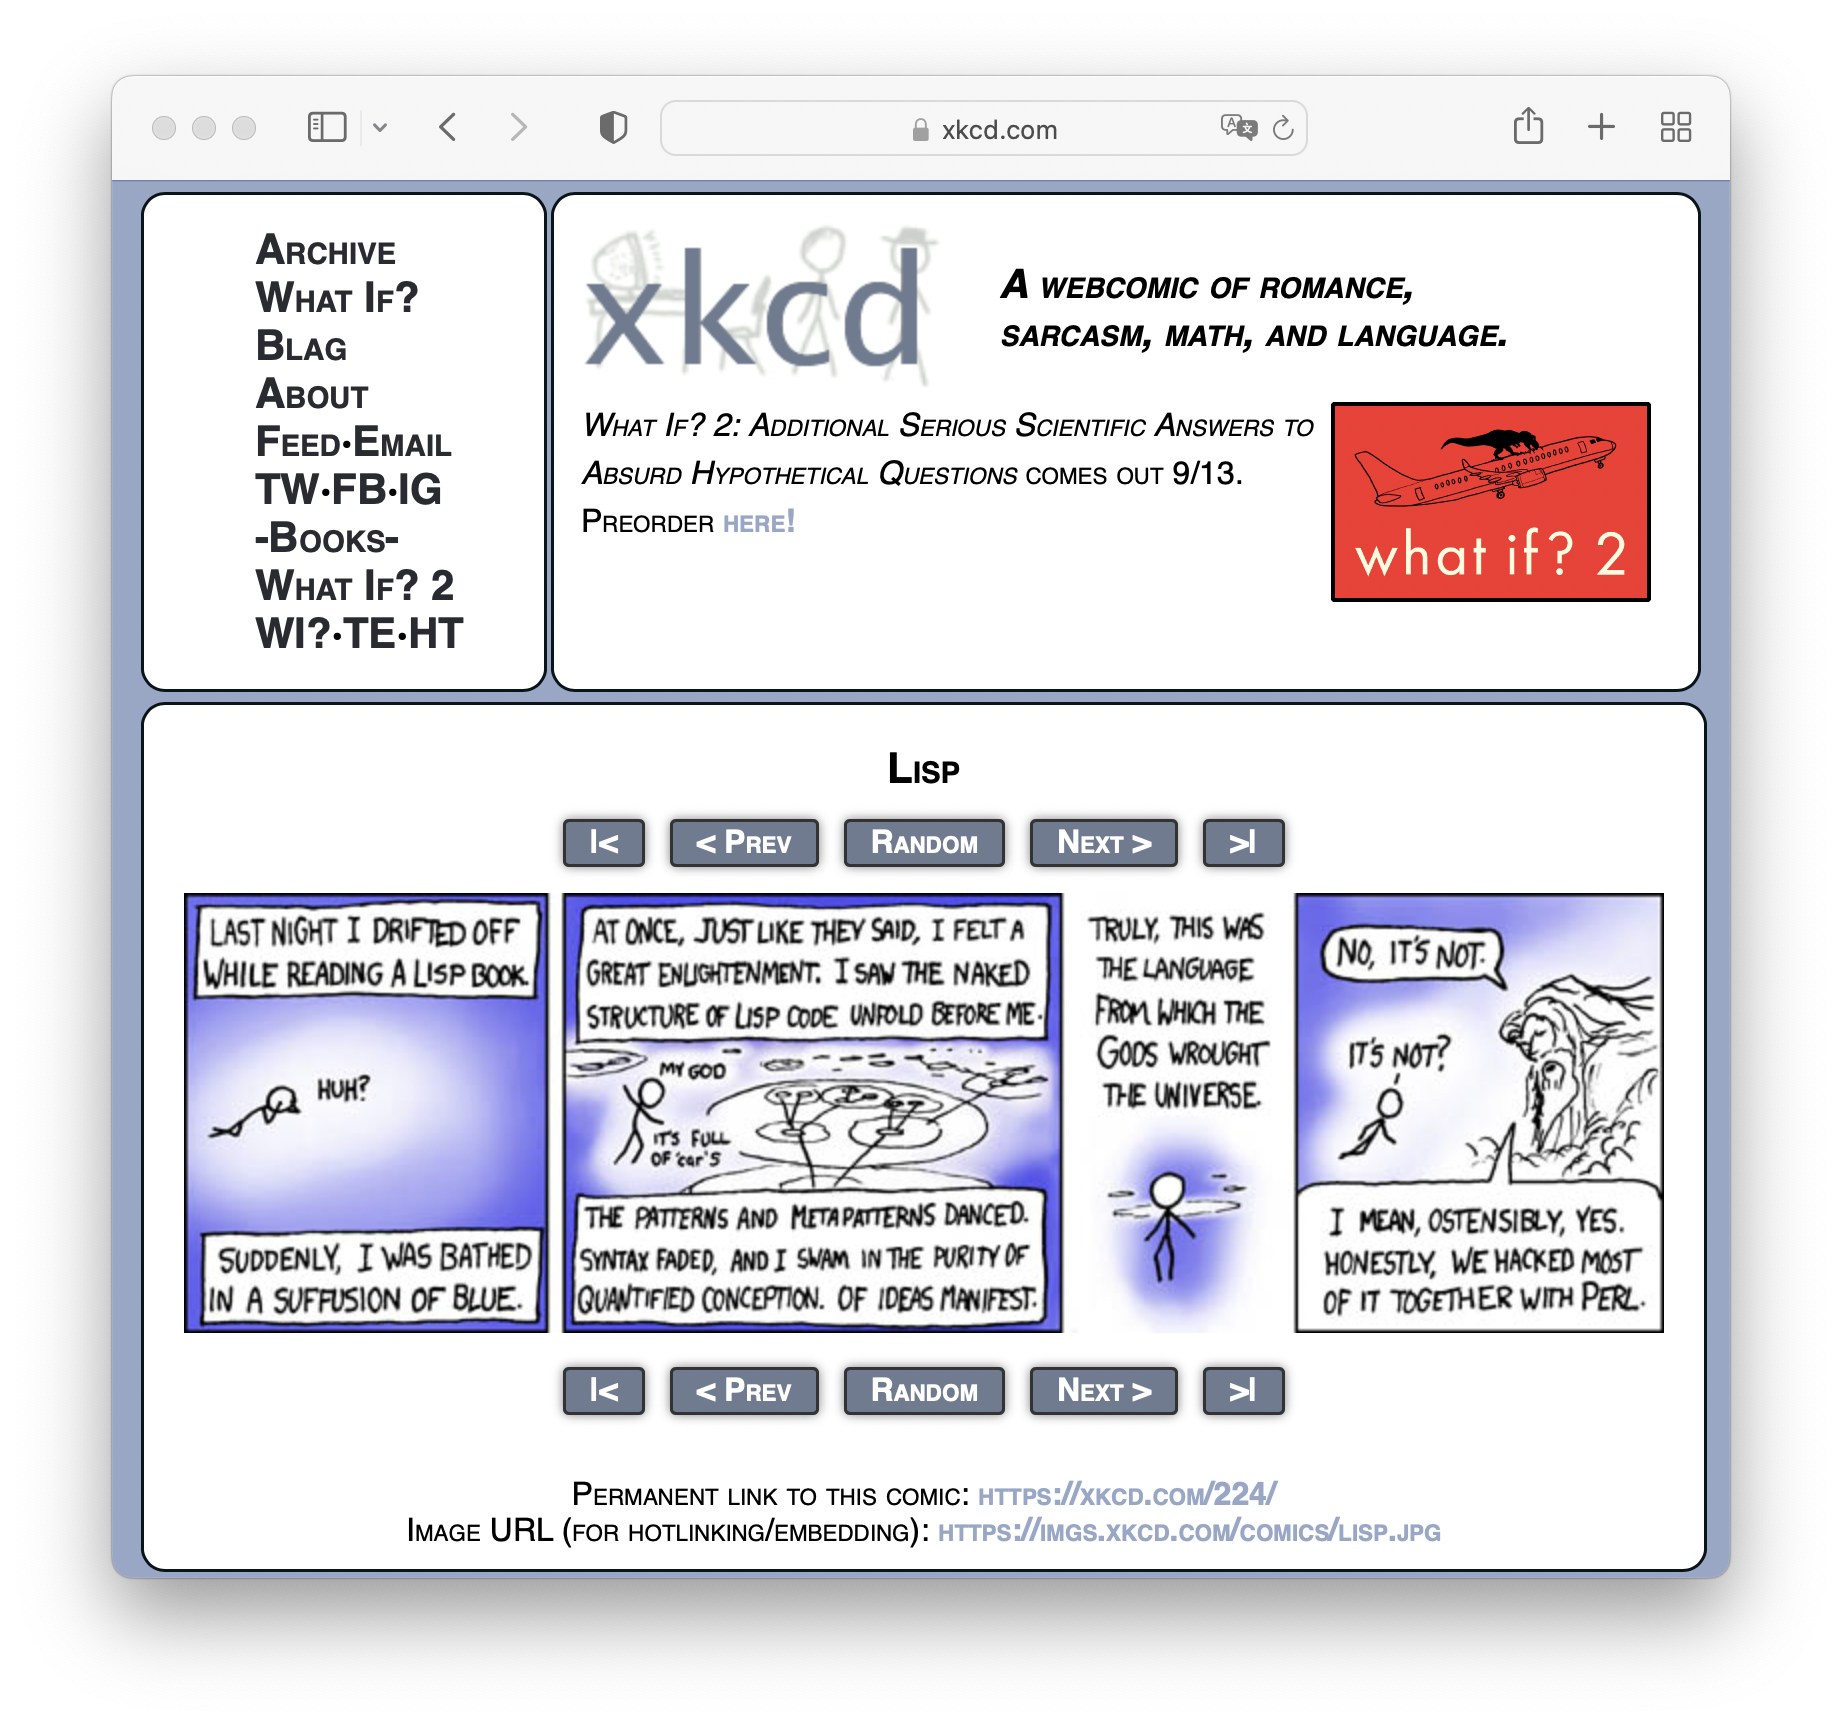
\includegraphics[width=0.75\textwidth]{image/chapter/1_language/xkcd.png}
%   \caption{xkcd的网页\footnote{2022/4/4的快照}, 注意下方有图片的地址哦}
% \end{figure}
% 
% 但是你会发现, 自己假如想要保存很多照片的话, 或者不是很想要自己来干活的话, 这个时候你就会想要说: 啊, 我想要能够自动化操作这些事情, 让这些呆头事情交给电脑来干活吧. 
% 
% \begin{quotation}
%   \begin{minted}{ruby}
%     # 导入一个能够帮助我们使用http协议访问网页的库
%     require "net/http"
% 
%     # 储存我们要访问的网页的地址
%     url = URI("https://xkcd.com/224/")
%     # 访问网页
%     response = Net::HTTP.get(url)
% 
%     # 在网页中按照图片链接的形式来找到链接的图片名字, 
%     # 并将其转换为字符串储存在image_name里面
%     image_name = response.match(/\w+\.jpg/).to_s
% 
%     # 打开一个图片名字的文件, 并写入文件
%     File.open(image_name, "w") do |f|
%       image_url = URI("https://imgs.xkcd.com/comics/#{image_name}")
%       f.write(Net::HTTP.get(image_url))
%     end
%   \end{minted}
% \end{quotation}
% 
% 让我们来一点点地解释上面的语句的意义吧: \footnote{注: 就像是页底注一样, 在Ruby代码里面也有注释, 凡是用\textbf{\#}开头的, 后面跟着的东西都是注释. 也就是不会被Ruby当作是代码来处理. }
% 
% 首先是第一段: \mintinline{ruby}{require "net/http"}这个是告诉我们要使用一个叫做\textbf{http}的在\textbf{net}这个大范围下面的一个库(也可以叫做gem\footnote{这个的原本的意思就是宝石, 是不是非常的形象? 因为有这些像宝石一样好用的库, 才让我们的软件开发变得非常的方便和快捷. }). 什么是库呢? 库实际上就是一种"站在巨人的肩膀上"的一种东西, 前人帮我们建立好了完善的库, 然后我们只需要按照规则和约定形式地调用就好了. 实际上是一种抽象的概念: 我们不必在意冰箱的内部构造, 不需要思考热力学的热机, 也不需要担心转轴和密封性. 只需要知道, 冰箱有一个门, 可以打开和关上; 冰箱里面可以放东西. 仅此而已, 就可以利用冰箱这样的神奇的东西. \footnote{但是这样的话我们就会失去对底层的了解, 假如我们想要造一台利用冰箱原理的冰库, 或者需要设计一个使用冰箱的制冷机技术的空调, 这时候我们就有必要了解如何hack掉那个压缩机才能进一步深入了. }
% 
% 我们所用的这个\textbf{net/http}库的作用就是可以方便地帮助我们通过HTTP协议来链接网页. 
% 
% 然后是第二段访问网页的操作: 首先是告诉Ruby, 要用一个变量\textbf{url}, 就像是名字(或者是外号)一样, 记下网页的地址并方便以后的使用. 然后告诉Ruby, 我们要用一个在\textbf{Net}里面的\textbf{HTTP}里面的方法\textbf{get}方法(method)来取得网页. 
% 
% 接下去那一段就是在网页的返回的内容里面找出图片, 我们使用了一种叫做正则表达式(Regexp)的方式来匹配有一定模式的文本, 具体的组织方式我们将会在之后介绍, 现在我简单地介绍一下: 上面的\mintinline{ruby}{/\w+\.jpg/}的功能就是用来匹配\textbf{文字.jpg}这样的东西. \footnote{不过假如你想要卷的话, 不妨了解一下: \href{https://ruby-doc.org/core-3.1.1/Regexp.html}{Regexp}, 学会看文档也是一种很有必要的技能哦. 虽然现在可以不了解, 但是以后还是建议掌握. }也就是我们的图片的名称. 
% 
% 最后是将这个图片名称变成链接, 然后保存在文件里面. 这里我们会看到一个使用\textbf{File}中的\textbf{open}方法来用写("w", 也就是write属性)打开, 简单记为\textbf{f}来方便我们在代码块里面使用. 最后往里面写\textbf{write}图片链接里面的内容呢. \footnote{我觉得还是很有必要介绍一下如何运行代码吧, 虽然我会在附录里面更详细地介绍. 简单来说, 就是将代码保存到文件(比如叫做\textbf{download\_pic.rb})里面, 然后在命令行里面输入命令 \textbf{ ruby download\_pic.rb } 最后就能够运行啦. 记得查看运行的目录里面是否有保存的图片文件出现哦. }
% 
% 上面的过程我们其实只实现了一个网页的下载, 那么我们接下来试试看下载更多的网页吧: 
% 
% \begin{quotation}
%   \begin{minted}{ruby}
%     # 导入一个能够帮助我们使用http协议访问网页的库
%     require "net/http"
% 
%     # 储存我们要访问的新的网页的地址
%     url = URI("https://xkcd.com/54/")
%     # 下面同理... 
%     response = Net::HTTP.get(url)
%     image_name = response.match(/\w+\.jpg/).to_s
% 
%     File.open(image_name, "w") do |f|
%       image_url = URI("https://imgs.xkcd.com/comics/#{image_name}")
%       f.write(Net::HTTP.get(image_url))
%     end
%   \end{minted}
% \end{quotation}
% 
% 我们会发现, 诶, 上面的代码不是和之前的代码几乎一模一样吗? 不过就是修改了一下新的\textbf{url}罢了. 假如有一种东西, 能够只需修改\textbf{url}, 就能够运行类似的过程就好了. 所以我们就要进入到一个抽象的概念中了: 
% 
% \begin{quotation}
%   \begin{minted}{ruby}
%     require "net/http"
% 
%     # 定义了一个方法(函数)
%     # 下载xkcd网站中对应链接的图片漫画
%     def download_image(link)
%       url = URI(link)
%       response = Net::HTTP.get(url)
%       image_name = response.match(/\w+\.jpg/).to_s
% 
%       File.open(image_name, "w") do |f|
%         image_url = URI("https://imgs.xkcd.com/comics/#{image_name}")
%         f.write(Net::HTTP.get(image_url))
%       end
%     end
% 
%     download_image("https://xkcd.com/54/")
%     download_image("https://xkcd.com/53/")
%     download_image("https://xkcd.com/52/")
%   \end{minted}
% \end{quotation}
% 
% 
% 于是, 我们相当于只需要一句话就能够调用原来的长长的一串命令. 在形式上看, 我们就像是告诉Ruby, 记下一个叫做\textbf{download\_image}的函数名字. 然后每次Ruby看到这个名字的时候, 就都会去"回忆"一下之前定义的函数的内容. 然后我们传递给函数的参数将会按照顺序告诉函数的代码块里面. \footnote{之后会详细介绍参数的使用方法的, 现在只需要知道我们的函数的参数都是按顺序传递的就好了. 唯一稍微需要注意的就是, 我们之前介绍的代码块(block)是在最后传递给函数的. }
% 
% 这个时候我们只需要使用"黑箱方法"就能够调用原本复杂的方法, 即不需要知道其中具体的实现和细节, 只需要知道宏观的外部的调用方法, 就能够使用该程序和函数了, 这就是黑箱方法. 这里就体现了一种抽象的概念: 我们将一个复杂的过程抽象成一个简单的结构. 就可以非常轻松地调用了. 

\section{Get Your hands dirty}
\begin{quotation}
  我的目的是想说明, 这一天空机器并不是一种天赐造物或者生命体, 它只不过是钟表一类的机械装置(而那些相信钟表有灵魂的人却将这一工作说成是其创造者的荣耀). 在很大程度上, 这里多种多样的运动都是由最简单的物质力量产生的, 就像钟表里所有活动都是由一个发条产生的一样. 
  
  约翰尼斯·开普勒(给Herwart von Hohenburg的信, 1605)
\end{quotation}

上面的故事里面, 我们只是在做类似于思想训练的东西, 没有接触很多实际的操作. 这怎么可以呢. 只是想想, 却不实际操作, 总觉得有一种画饼的意味. 所以接下来我们来实际地接触一些实际的东西. 

(又: 我现在觉得实际的东西还是在迟一点点来吧, 下面的东西请务必操作\footnote{关于操作的问题, 建议使用irb(Interactive Ruby)来操作. 关于这个, 可以看看我的这个\href{https://li-yiyang.github.io/ruby/why's_(poignant)_guide_to_ruby/why's-poignant-guide/}{翻译}. 之后会在附录中加入一些关于这个irb的介绍的. }试试看. )

\subsection{用你的名字呼唤我}
\begin{quotation}
  O Romeo, Romeo, wherefore art thou Romeo?

  Deny thy father and refuse thy name.

  Or if thou wilt not, be but sworn my love

  And I'll no longer be a Capulet.

  `Tis but thy name that is my enemy:

  Thou art thyself, though not a Montague.

  What's Montague? It is nor hand nor foot

  Nor arm nor face nor any other part

  Belonging to a man. O be some other name.

  What's in a name? That which we call a rose

  By any other name would smell as sweet;

  So Romeo would, were he not Romeo call'd,

  Retain that dear perfection which he owes

  Without that title. Romeo, doff thy name,

  And for that name, which is no part of thee,

  Take all myself.

  \emph{from Romeo and Juliet, spoken by Juliet}
\end{quotation}

但是我不觉得名字不是很重要, 每一个优秀的巫师都知道真名\footnote{乐, 其实这个的真名更像是地址. 在我们熟悉的递上苹果的蛇的后裔之一 -- Python 中, 变量储存的就是值的地址的引用. }的重要性. 罗密欧抛弃了他的"名字", 但是他的自身并不会被因此抛弃. \footnote{这个我们可以用Python的变量来看看, \mintinline{python}{name = "Romeo"; new_name = name; id(name) == id(new_name) # => True}, 这个时候我们就会看见, 哪怕变量的名字不同, 只要它们指向的东西是一样的, 那么它们的identify(id)就都是一样的. 呃, 这个有点没意思, 因为Python的变量还是和C的指针有点区别, 这里看不懂没关系, 就跳过吧. } 倘若连自身的值(ego)都给扔了, 那么等待他的就只有被GC(垃圾回收机制)给消除的命运了. 

乐, 还是不要在意这些东西了, 让我们给他一个新的名字吧. 

\begin{quotation}
  \begin{minted}{ruby}
    name = "Romeo"
    price_of_the_sword = 1_000_000
    the_name_of_my_kitty = "Lucky"
  \end{minted}
\end{quotation}

上面就是一串的命名的过程. 我们通过形式化的一个\textbf{名字 = 值}的一个表达式来告诉Ruby, 我们要给这些值起一个名字, 其中值就是等号右边的内容, 名字就是等号左边的东西. 这样的表达式我们叫做赋值表达式. 

在地海传奇里面, "当知晓了某物/人之真名时, 便能成为其主人. "; 我们没必要使用那么大的杀器, 我只想在呼唤kitty的时候它能够回应一下. \footnote{但是我并没有小猫, 虽然我喜欢他们. } 那么在我们Ruby里面, 每一次我们喊出变量的名字的时候, Ruby就会帮我们找到那个变量名字对应的值, 然后拎起kitty的后颈, 把它轻轻地提到我们的面前. 

\begin{quotation}
  \begin{minted}{ruby}
    print "Where are you? ", the_name_of_my_kitty, " Come here! \n"
    print "Oh, yes! Here you are, my ", the_name_of_my_kitty
    # =>
    # Where are you? Lucky Come here!
    # Oh, yes! Here you are, my Lucky
  \end{minted}
\end{quotation}

(在上面的代码里面, 我们用\#号来表示注释, 所有在\#后面的东西都不会被Ruby看到, 所以我们用它来做一些小笔记. 就像不能被老师看到的小抄一样. )

并且就像我们给东西取名字的时候, 要有一定的规则, 不能随便乱起名字, Ruby里面, 给变量取名字也是一种小有学问的东西呢. 比如说, 我们不能够把名字取得让人混淆: \mintinline{ruby}{2333_is_not_a_variable}, \\\mintinline{ruby}{"name"_is_also_not_a_variable}, \mintinline{ruby}{:p_not_variable_name}, 这样的名字会让Ruby在阅读的过程中内心发出一堆的怀疑. 因为在Ruby看来, 这样的名字更像是数字, 字符串, 符号而不是变量名字, 但是后面跟着的东西有不像是数字, 字符串, 符号之类的东西, 这可真是让人头大. 所以Ruby就会非常生气地说我不干啦, 你好像出错了! \footnote{这个时候会报错: \textbf{SyntaxError}, (以\textbf{2333\_is\_not\_a\_variable}为例, 其他的你可以试试看)如果我们来尝试阅读一下报错的信息的话, 就会发现Ruby看到开头的数字就会认为是数字, 而看到紧跟的奇怪东西, 就会感到困惑, 最后爆出错误: \\ SyntaxError ((irb):*: trailing `\_' in number)\\(irb):*: syntax error, unexpected local variable or method, expecting end-of-input} 所以我们起名字的时候, 还是老老实实地取一个不是那么古灵精怪的名字吧. 比如说\mintinline{ruby}{a_good_name}, \mintinline{ruby}{the_name}, 之类的名字吧. \footnote{虽然数字之类的也是可以用在变量名字里面的, 比如\mintinline{ruby}{var_233}之类的, 但是怎么说呢, 看到这种带数字的名字, 我常常会感到十分的头疼. \mintinline{ruby}{v1, v2, v3}这样的东西写起来和看起来都像是在糊弄, 所以我不在正文里面介绍, 也不希望你学习, 因为这样的代码真的很难看. }

不知道你有没有发现, 很多专有名词名词在英文里面都是用大写字母开头的, 比如\textbf{China}, \textbf{English}, \textbf{German}之类的. 没错, 在Ruby里面, 我们也用大写开头的"变量"名字来表示一种"专有"的特色. 就像"一个中国"是不可动摇的原则一样, 用大写开头的"变量"名字也就像是在捍卫自己不可更改的坚定立场. 所以我们叫这样的量为常量. 不过Ruby也不是那种死脑筋, 假如你想要修改一个常量, 也不是不行. 因为这个是科学, 科学允许质疑, 否则你得到的只有教条. \footnote{比如说关于电子的荷质比的测量. 密立根油滴实验做的事情就比较坑爹了. 不仅卖了自己的学生, 还做了筛选数据的操作(让数据变得符合他的喜好). 导致了因为自己的诺贝尔奖, 把这个重要的科学常数的精确值的测量推迟了许久. 但是科学厉害之处就在于它是可以质疑, 不断修改精进的. } 只是Ruby会给你一个提示: "warning: already initialized constant", "(irb):line: warning: previous definition of Constant\_Name was here". 不过你还是最后能够修改常数的值啦. 

\begin{figure}[h]
  \centering
  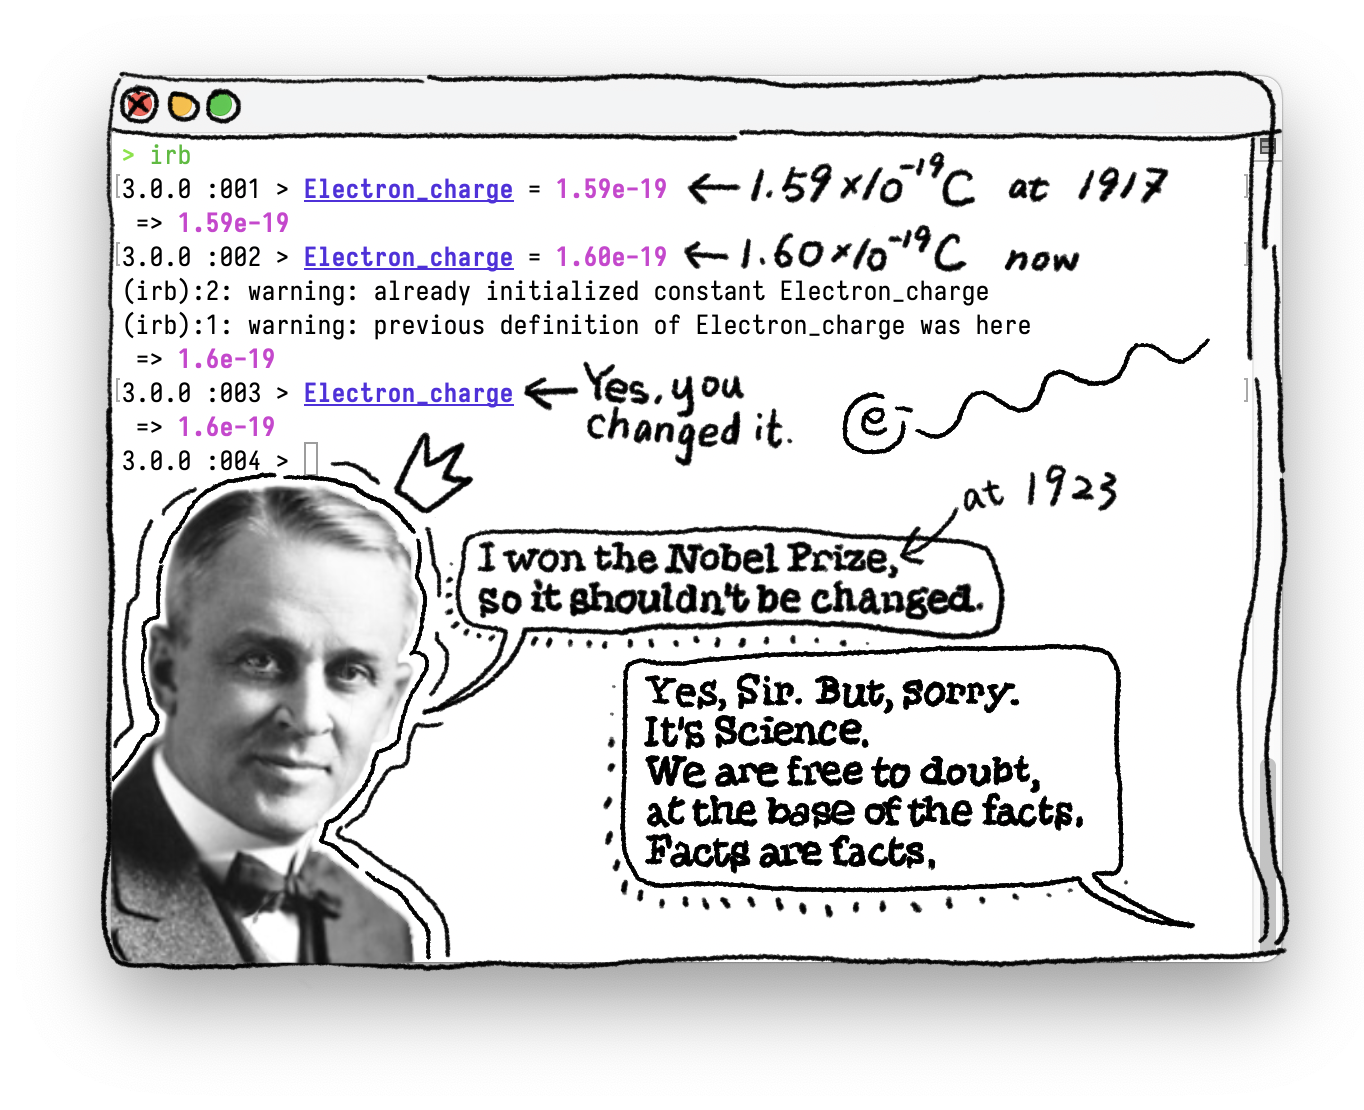
\includegraphics[width=0.75\textwidth]{image/chapter/1_language/constant.png}
  \caption{常量也是可以改的}
\end{figure}

于是, 当我们想要把一个值保存起来, 然后以后再调用的话, 就可以利用赋值语句来实现我们的目的了. 在这个过程中, Ruby会将这些名字保存在自己的一个小册子里面, 然后每次见到一个看起来像是名字的时候, 就会去这个小册子里面翻找 -- 对了, 为什么不先看看这个神奇的小册子呢? 

(在irb中: )

\begin{quotation}
  \begin{minted}{ruby}
    local_varibles
    # => [:the_name_of_my_kitty, :price_of_the_sword, :name, :_, :version, :str]
  \end{minted}
\end{quotation}

可以看到, 在\textbf{local\_varibles}这个名字\footnote{其实是一个方法的名字}里面, 储存了我们的变量的名字. \footnote{这里是用Symbol类型来记录的. 又, 这里是一个无关紧要的小注释, 为什么要用Symbol而不是String呢? 这是因为相比容易可以发生变化的String, Symbol不太容易发生变化, 并且在比较和调用的时候比较快. 也就是说, 当你想要标记但是又不是很想打印的时候, 使用Symbol就是一个比较好的选择. } 但是假如我们访问了一个不存在于这个小册子里面的变量的时候, 就好像有人突然在你面前提到了一个你从来没有听过的名字, 这个时候, Ruby就会正直地提示你: 

\begin{quotation}
  \begin{minted}{ruby}
    an_undefined_name
    # => 
    # Traceback (most recent call last):
    #     4: from irb:*:in `<main>'
    #     3: from irb:*:in `load'
    #     2: from irb:*:in `<top (required)>'
    #     1: from (irb):*:in `<main>'
    # NameError (undefined local variable or method `an_undefined_name' 
    # for main:Object)
    an_undefined_name = "Hey, Ruby, this variable is such a thing. "
    an_undefined_name
    # => "Hey, Ruby, this variable is such a thing. "
    local_variables
    # => [:an_undefined_name, :x, :the_name_of_my_kitty, 
    # :price_of_the_sword, :name, :_, :version, :str]
  \end{minted}
\end{quotation}

可以看到, 这里Ruby在最后告诉你出现了一个\textbf{NameError}, 也就是对你的这个名字, Ruby会说, 嗯, 这个名字好像我没有见过. 当我们在Ruby里面定义了这个名字之后, 再次调用这个名字的时候, Ruby就知道了该拿什么了. 

众所周知, 情人眼里出西施. 罗密欧的眼里的"西施"是朱丽叶, 但是在其他人眼中的"西施"可就不一定是朱丽叶啦. 这就像是"一千个人眼中有一千个哈姆雷特"一样, 在不同的区域里面的变量可能会有不同的意义. 

在Ruby里面, 我们就有类似的"区域"的概念. 比如说我们在前面遇到过的代码块结构(\textbf{do...end}), 或者是我们见到过的定义方法的结构(\textbf{def name ... end})\footnote{以及在之后我们会遇到的Module, Class等的东西}等等. 在这里, 我只会简单地介绍一下这个"区域"的概念, 至于更加复杂的问题, 恕我先搁置一边啦. 

不知道你有没有玩过显微镜(其实望远镜也是一样的, 只是我没有玩过望远镜), 当我们选择了一个镜头看到了一堆 -- 比方说洋葱表皮细胞吧 -- 时, 你可能会感慨, 哇哦, 好厉害的细胞, 好漂亮的玩意儿! 然后, 为了更好地看清楚这些细胞, 你换上了一个更大放大倍数的物镜(嗯, 轻轻地旋转你的转换器, 不要让镜头压到你的载玻片), 这个时候, 你的视野聚焦在了一个更加精细的区域, 原来的密密麻麻的细胞们全部都从镜头的中心离开了, 只留下一个主角. 

Ruby中的"区域"就像是这样的东西. 这也就是为什么它的正式名字叫做\textbf{Scope}(显微镜的英文名字叫做mircoscope). 那么我们现在来一点点例子吧: 

(在一个新的irb进程里面: )

\begin{quotation}
  \begin{minted}{ruby}
    a_variable = "This is a variable"
    another_variable = "Oh, This is an other variable"
    def test_method
      a_variable_inside_method = "This variable is inside method"
      another_indside_variable = "Inside variable are not available outside"
      print local_variables
    end
    test_method
    # => [:a_variable_inside_method, :another_indside_variable]
    local_variables
    # => [:another_variable, :a_variable, :_, :version, :str]
  \end{minted}
\end{quotation}

上面我们就会发现, 在方法\textbf{test\_method}中的变量不是在外面的变量, 在外面的变量也不能够在方法中调用, 就好像是我们将显微镜的镜头对准了一个新的区域, 观察完后回到了原来的过程中. 于是在观察这个新的区域中时, 我们没法知道原来的区域里面有什么, 回到了原来的区域中后, 我们也不知道新的区域里面有啥. 这个时候, 我们就叫这样可以分别储存变量的区域叫做命名空间(NameSpace), 因为在里面我们可以自行命名东西而不用顾及其他命名空间. 

再来一些例子: 

\begin{quotation}
  \begin{minted}{ruby}
    x = 2333
    def print_x
      print x
    end
    print_x
    # => 
    # Traceback (most recent call last):
    #     5: from irb:*:in `<main>'
    #     4: from irb:*:in `load'
    #     3: from irb:*:in `<top (required)>'
    #     2: from (irb):*:in `<main>'
    #     1: from (irb):*:in `print_x'
    # NameError (undefined local variable or method `x' for main:Object)
  \end{minted}
\end{quotation}

上面的例子体现了不同的命名空间的名字是不通用的, 其实这个原因是因为在\textbf{print\_x}方法中的local\_variables里面, 没有x的名字. (僕わ知らない、君の名前, 乐)

(呃, 上面那一部分写的不是很好, 所以之后再想办法优化, 现在不想写了. )

但是这个时候就出现了一个问题, 假如一个意气风发的家伙狂妄自大地高喊, 啊, 我的话语是真理, 所有的人眼中的真理都该是我所说的话语, 我即是自由与民主... 那么这个人一定也会很反感"一千个人眼中有一千个哈姆雷特"的说法. 但是这个家伙太精明了, 他用金钱武装起自己的话语, 在全球分发传播自己的话术, 遇到阻碍就用金钱在前方开道, 于是他的话术就传播到了各个角落, 成为了"真理". 不过Ruby没有这么黑暗和腐败, 只是作为一种戏谑, 我们定义了一种类型的变量, 它们在命名的时候用美元符号(也就是金钱)开头, 然后不论是在那个角落, 这样的变量都是一样的. 

举个例子: 

\begin{quotation}
  \begin{minted}{ruby}
    $what_mr_k_said = "I'll make world great again! "
    $what_mr_k_did = "I just made the world worse first"
    def people_in_area_A
      print "This is what Mr.K said: ", $what_mr_k_said, "\n"
      print "This is what Mr.K did: ", $what_mr_k_did, "\n"
    end
    def people_in_area_B
      print "据说K先生说: ", $what_mr_k_said, "\n"
      print "他做了: ", $what_mr_k_did, "\n"
    end

    people_in_area_A
    # => This is what Mr.K said: I'll make world great again! 
    #    This is what Mr.K did: I just made the world worse first
    people_in_area_B
    # => 据说K先生说: I'll make world great again! 
    #    他做了: I just made the world worse first
  \end{minted}
\end{quotation}

果然, 用金钱开道的话, 所有的区域的人都知道这位意气风发的先生所说的东西了. 

欸, 我们还是抛开这种低俗的打趣笑话吧, 我认为这样的东西没有什么意思. 除了让人哈哈大笑之外, 完全没有任何的营养. 还是回到竹林或者书斋之中, 培养一颗宁静的心吧. 

\begin{quotation}
  人皆有不忍人之心. 先王有不忍人之心, 斯有不忍人之政矣; 以不忍人之心, 行不忍人之政, 治天下可运之掌上. 

  \emph{《孟子·公孙丑上》}
\end{quotation}

假如孟子会一点点编程的话, 那么他一定会想说: 

\begin{quotation}
  \begin{minted}{ruby}
    class Human
      @@common_character = :kind_heart
      def initialize(name)
        @name = name
      end
    end
  \end{minted}
\end{quotation}

那么对每个\mintinline{ruby}{Human.new("张三")}以及\mintinline{ruby}{Human.new("李四")}, 那么在上面的代码中, 所有的\textbf{Human}类的对象都共同拥有一个变量名字叫做\textbf{common\_character}, 也就是每个人都应该有的共同的品质都是一颗不忍人之心. 但是每个Human类的对象, 也就是每个人可以有不同的\textbf{name}(名字). 

可能你觉得有点奇怪, 这两个变量和我们之前的变量有什么区别呢? 不就是变量名字前面多了一些奇怪的前缀 -- 没错, 就只是这样, 在形式上的前缀标志就表示了变量的"类型". \footnote{这个类型不是像String, Integer之类的值的类型, 而是全局变量, 类变量, 实例变量, 局部变量等等的变量类型. } 

你可以这样想: \footnote{我在这里只会简单定性地介绍, 暂时不会深究这些变量的具体实现. 建议你先是知道有这么个东西, 然后在之后我们会从一些比较基本的方向来介绍. } 

前面的全局变量(global variable), 因为它们前面拿着一个美刀符号(\$), 于是所向披靡, 在各个地方都是适用的. \footnote{和\textbf{local\_variables}的方法一样, 我们可以通过\textbf{global\_variables}这个方法来得到我们进程中的全局变量. 比如说在一个全新的irb里面, global\_variables方法的返回值为\mintinline{ruby}{[:$VERBOSE, :$-v, :$-w, :$-W, :$DEBUG, ...]}}

对于前面带了一个艾特号(@)的实例变量(instance variable), 你不妨把这个符号想象成一个小小的回形针, 轻轻地别在我们的实例对象(instance object)\footnote{等等, 你是不是想问我什么是实例对象? 其实这个就是我们之前一直说的对象啦. 只不过实例对象的这个名字更加注重强调对象是某个类的对象. 这个是一个叫做面向对象编程的思想的概念, 不过我建议您还是}上, 对象走到哪, 就带着这个实例变量来到哪里, 也就是说, 实例变量的作用区域就是我们的这个实例对象. \footnote{同样的, 你也可以\textbf{instance\_variables}来访问当前的对象的实例变量. 比如\mintinline{ruby}{Human.new("Lucky").instance_variables}就会返回\mintinline{ruby}{[:@name]}的结果. }

而前面有两个@@符号的类变量(class variable), 除了和实例对象相连以外, 还和类(class)\footnote{类其实也是一个对象, 在Ruby里面. }相连. 所以只要是同一个类的实例对象, 那么它们就都共同分享着同样的类变量. \footnote{没错, 你没猜错我们还是能够用简简单单的一个method来访问类的变量, 就决定是你啦: \mintinline{ruby}{Human.class_variables}, 这条命令的返回结果就是\mintinline{ruby}{[:@@common_character]}. }

对于那些普普通通的变量(local variable), 没有任何的前缀, 只能够在一个小小的区域里面随风飘扬. 不过对于代码块之类的在局部查找变量的东西, Ruby还是能够找到它们的. 然而一旦你换到了一些新的区域的时候, 我们就不知道该怎么找到他们了. 

这个并不是Ruby真正的实现方法, 但是假如我们想要实现一个类似的储存变量的方法的话. 这里提供一个简单的想法: 假如我们学过一点点物理的话, 我们就会想到, 嘿, 所有的参考系都应该是平等的, 好像没有什么"绝对"参考系吧. 所以要确定一个物体的位置, 我们总是要去寻求相对位置来找到. 同样的, 我们可以利用相对位置来实现变量的引用, 比如假如我们的区域是一张表格: 

\begin{figure}[h]
  \centering
  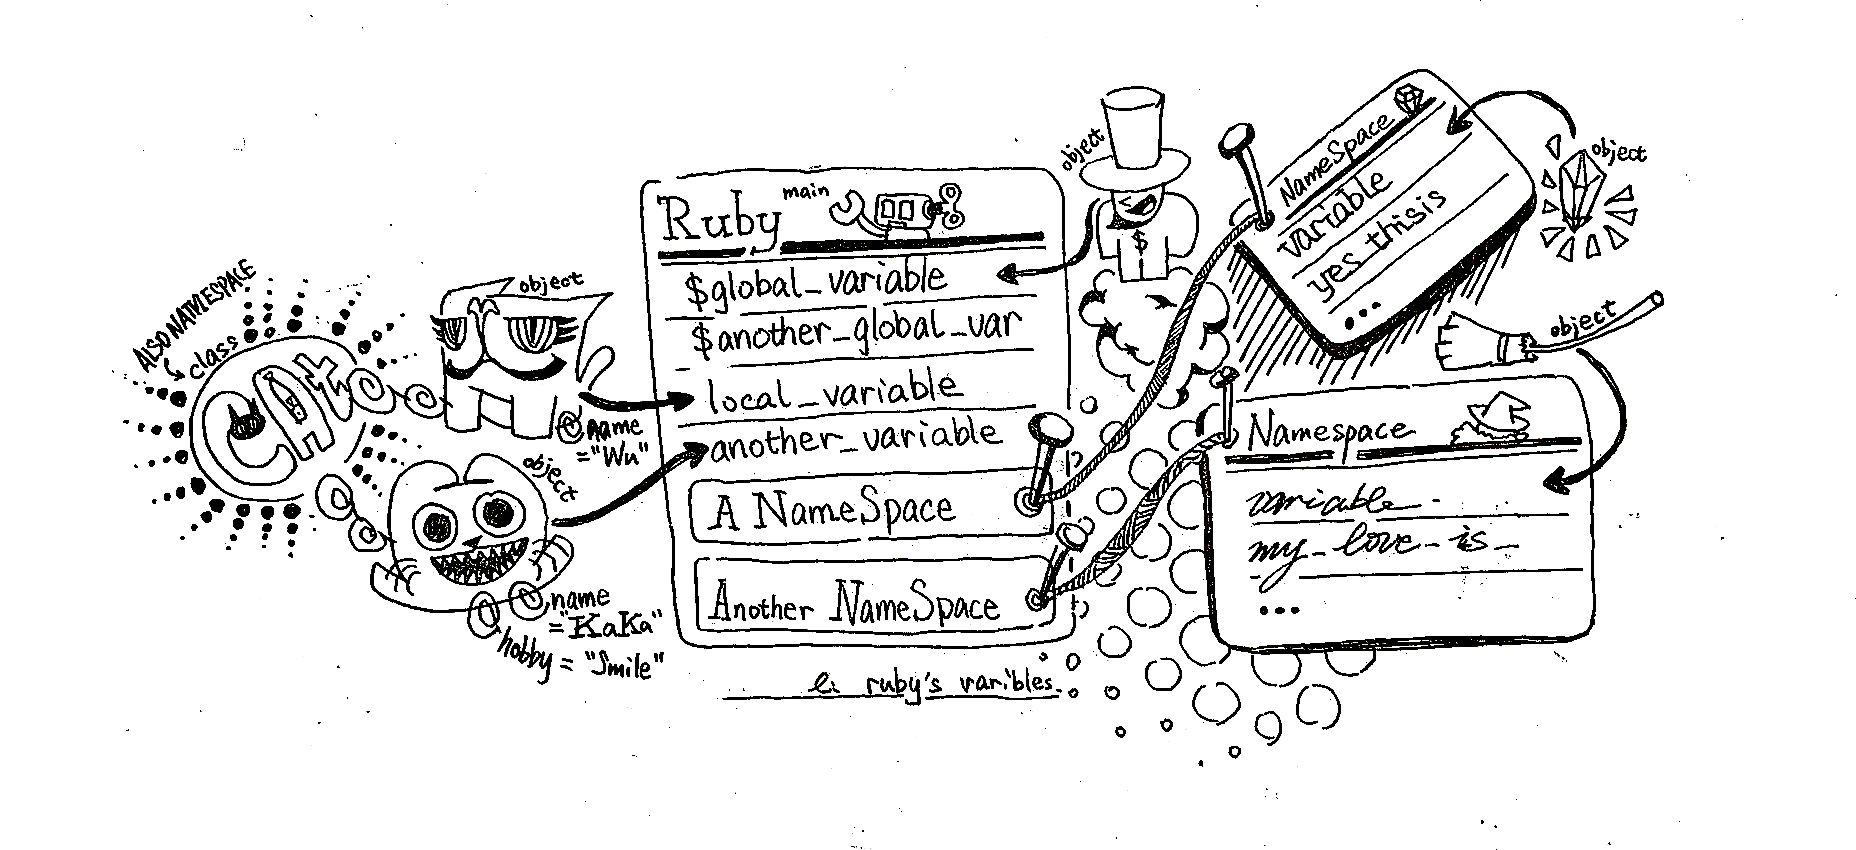
\includegraphics[width=\textwidth]{image/chapter/1_language/ruby_variables.jpg}
  \caption{Ruby的变量们}
\end{figure}

当我们想要访问一个变量的时候, 我们就会在当前所在的命名空间里面去寻找, 除非是看到了用\$号开头的全局变量, 才会去约定的地方去寻找. 而我们的实例变量则是相对着实例对象来找的. \footnote{这也就是为什么你会常常看到Ruby里面有类似于有\mintinline{ruby}{object.instance_variable_name}的玩意啦. }而类变量则相对着类来寻找. 这里我们就体现了一种寻找变量值的想法啦. \footnote{具体的话, 我们会在之后再进行一个介绍, 如果可以的话, 我们没准还能实现一个呢. } 这里的寻找变量的方式就是一种相对位置的想法啦. 

那么总结一下

嗯, 我们关于赋值的问题就介绍到这里. 接下来, 让我们抛开赋值的这些乱七八糟的约定. 可以发现, 我们的赋值的操作让我们能够将值和(变量)名字联系在一起, 只需要呼唤名字, 就能够调用原来的值. 或者是更新, 替换, 修改原来的值. 比如: 

\begin{quotation}
  \begin{minted}{ruby}
    string = "I'm the King of the "
    string = string + "Nuts"
    string
    # => "I'm the King of the Nuts"

    string.upcase
    # => "I'M THE KING OF THE NUTS"
    string.downcase
    # => "i'm the king of the nuts"

    my_money = 100
    price_of_cookie = 10
    my_money -= price_of_cookie
    my_money
    # => 90
  \end{minted}
\end{quotation}

这样我们就得到了存放数值的能力, 并且也可以用一个名字来抽象地调用这个值, 从而实现更加强大的功能. 可惜我比较笨, 这里就写一个很普通的利用存放数值的特性交换的例子来结束我们的这一小节吧: 

想象一下, 一个莫得感情的杀手, 为爱杀了人, 从此浪迹天涯, 流落他乡. 一个小女孩委托人, 泥沟里翻滚的父母将她的命运拖入了深渊, 渴求着复仇的她委托杀手替她报仇. 看着小女孩, 杀手的心松动了, 警醒让他明白这样的后果, 人性让他走向了那没有回头路的灭亡之路. 所以他把自己的积蓄留在了线人那里. 他知道自己终将失去, 只是希望至少能够让那个小女孩能够拥有自由的生活. 于是他用自己的至宝与小女孩的一无所有交换, 

\begin{quotation}
  \begin{minted}{ruby}
    leon = "Leon's Treasure"
    mathilda_lando = "Nothing"

    old_tony = leon
    leon = mathilda_lando
    mathilda_lando = old_tony
  \end{minted}
\end{quotation}

上面的代码我们就利用了一个存放数据的概念来做了一个交换, 一开始, 两个变量手中有着各自的值. Léon将自己的值交给了中间人Old Tony, 然后拿起了Mathilda Lando的值. 而Mathilda Lando则从中间人那里拿到了Léon曾经的值. 于是交换过程结束. 我们利用了一个中间变量来实现了两个变量之间值的转换. \footnote{虽然我们还有更多的转换方法, 其中Ruby提供了一个非常酷的方法: \mintinline{ruby}{leon, mathilda_lando = mathilda_lando, leon}, 不过这个代码的背后也有中间变量. 不过是Ruby自动为我们生成的. 为了理解这个, 我们还有一些路要走(因为我不打算接下去将数值类型), 所以放在脚注里面. }

\subsection{高速吟唱魔法咒语的什么的真是受够了}
想象一下人头攒动的庙宇中烟雾缭绕, 本就昏暗的庙堂因此更加声明而难以看清四周. 身边传来楠楠的祷告声, 人们念着自己的心愿. 台上的法师的言语穿过烟雾和人声, 更加得遥远和神秘, 本就听不清楚的祷告声变得更加的让人迷幻了: \footnote{这一篇我打算以传统的祈雨仪式为例子. (原因是因为之前看到了一篇韩愈的祈雨文, 可惜不知道叫什么了. 后来找到了杜牧的祭文. 本来想要删掉的, 因为太多了, 最后我觉得还是保留下来吧. 还有一本专著叫做《從人間世到幽冥界: 唐代的法制, 社會與國家》不过没有看过. ) 只是在网络上搜索相关的资料发现简直是寥寥无几, 并且也没有很详细的介绍. 大多是那种概括性的文字, 果然还是应该要找到那种一手资料吗. 不过通过这次的尝试, 我发现了自己的不足了. 果然还是缺少一些积累吗. }

\begin{quotation}
  下土之人, 天實有之. 五穀豐實, 寒暑合節, 天實生之. 苗房甲而水湮之, 苗秀好而旱莠之, 饑即必死, 天實殺之也. 天實有人, 生之孰敢言天之仁, 殺之孰敢言天之不仁. 刺史吏也, 三歲一交. 如彼管庫, 敢有其寶玉;如彼傳舍, 敢治其居室? 東海孝婦, 吏寃殺之, 天實寃之, 殺吏可也. 東海之人, 於婦何辜, 而三年旱之? 刺史性愚, 治或不至, 厲其身可也, 絕其命可也!吉福殃惡, 止當其身. 胡為降旱, 毒彼百姓? 謹書誠懇, 本之於天, 神能格天, 為我申聞. 

  \emph{杜牧《祭城隍神祈雨文》}\footnote{对不起杜牧先生, 我拿你的文字来作为例子了. 但是前面引入例子的文字实在是写得一般了. \\ 我在\href{https://m.djol.org/show-34-11627-1.html}{网络(不过建议还是不要访问, 因为看起来不正规)}上找到了一个比较像是的东西, 但是我觉得还是不如杜牧的好: \\
  伏以. 玄穹高上玉皇大帝并雷公, 电母, 风伯, 雨师四大雨神. 兹为**流域祈求甘霖缓解旱情而文. 雨神居上阙而管下界之水, 黎民居下界而仰上京之神, 上神赐福于黎民, 则黎民敬仰上神, 上神无视于黎民, 则黎民不信上神. 上下相关, 神民相依也. 尝曰:民以食为天, 食以粮为主, 粮以水为本. 无粮则人不存, 无水则粮不生. 今春以来, 上苍惜雨, 下界无流, 大河缩萎, 小河干涸, 田地豁裂, 庄稼枯黄, 江汉流域, 尤为其甚. 早稻因无水而少插, 中稻因无水而损苗. 时下已是中稻移栽旺季, 斯地依然干旱少雨, 无水整田. 百姓惶惶, 仕宦忧忧. 今弟子施惠奏明太上, 获准向天庭求雨, 以解斯地旱情, 保中稻栽插, 解燃眉之急, 润十方之农田, 更润百姓之心田. 恳望玉帝并四大雨神, 三日之内, 为上述旱区普降甘霖. 则百姓感上神之大恩, 三界记上神之大功. **道人 顿首叩拜}
\end{quotation}

概括一些就是: 

\begin{quotation}
  乞雨女郎魂, 炰羞洁且繁. 庙开鼯鼠叫, 神降越巫言. 

  旱气期销荡, 阴官想骏奔. 行看五马入, 萧飒已随轩. 

  \emph{韩愈《郴州祈雨》}
\end{quotation}

\begin{quotation}
  汤既克夏, 大旱七年, 洛川竭. 汤乃以身祷于桑林, 剪其发, 自以为栖牲. 祈福于上帝. 于是大雨总至, 洽于四海. 

  \emph{《搜神记·变化篇》}
\end{quotation}

你看, 我们可以用一些非常简明的文字来表述那些复杂的事情. 仅仅通过概念来感受这样的祈雨的氛围. 甚至这种仅仅通过概念来传递表示的能力能够超越时空, 哪怕是自己可能从来没有类似的体验的东西, 也能够通过概念的方式来理解和传递. 这里就是一种抽象的概念. \footnote{什么是抽象呢? 举个例子, 假如你的同桌搞了一支很有意思的自动铅笔, 然后借给你看看, 你抚摸着笔的外壳, 比较光滑; 笔握部分的橡胶也比较舒服; 出芯和书写也非常的快乐. 这个时候, 你是通过感官的表象来感受认识"笔"的. 但是有些时候, 你却并不能够直接通过直观或者感官来直接感受, 就像我现在是通过文字来间接的触动你的神经来产生对那支笔的认识. 这个时候就出现了一种抽象的感觉 -- 即我们不再是通过表象, 而是抽象的概念来认识一个东西了. 甚至, 哪怕这只笔已经不复存在了, 甚至只是我臆造的一个概念, 你也能够产生相应的认识. }

对于计算机来说, 抽象也是一种非常重要的一种东西. 我们之前其实就已经见识了抽象的一种了: 变量. 我们通过变量这一种抽象的概念, 用变量的名字来抽象地访问一个值. 这个时候, 我们不再是具体地处理数值, 而是通过名字来形式地调用. 

这一次, 我们将会不仅仅停留在对数值的抽象, 而是进一步深入, 来看一看更加有趣的对过程的抽象吧. 

比方说我们现在有一个非常复杂的过程: (注: 我的目的不是为了分析这个又臭又长的烂程序, 所以不要计较里面的具体做法和实现. )

\begin{quotation}
  \begin{minted}{ruby}
# 一周有七天
7.times do |day|
  # 每天十一节课
  11.times do |index|
    # 在网页中找到那一节课的信息
    box = file.xpath("//tbody/tr[#{index + 1}]/td[#{day + 1}]/div/a")
    # 假如这节课不是空的
    unless box == []
      # 有时候同一节课的时间会有不同的课
      box.each do |item|
        # 得到课程的链接
        link = item.xpath("@href").text
        # 得到课程的信息
        course_data = get_info(link, day)
        # 对于相应的课程
        course_data[:opening_week].each do |week|
          # 计算日期, 还有其他一堆东西
          date = start_date + 7 * (week.to_i - 1) + day
          the_year = date.year
          the_month = date.month
          the_day = date.day
          sthour = TIME_MAP[index][0][0]
          stmin = TIME_MAP[index][0][1]
          edhour = TIME_MAP[index][1][0]
          edmin = TIME_MAP[index][1][1]
          # 往日历中加入课程的信息
          cal.event do |event|
            event.dtstart = DateTime.civil(the_year, the_month, the_day, sthour, stmin)
            event.dtend = DateTime.civil(the_year, the_month, the_day, edhour, edmin)
            event.summary = course_data[:summary] + "-" + course_data[:location]
            event.alarm do |alarm|
              # alarm.summary = "Go To Class!"
              # 提前提醒
              alarm.action        = "AUDIO"
              alarm.trigger       = "-PT#{BEFORE_MIN}M"
              alarm.append_attach "Chord"
            end if BEFORE_MIN != 0
          end
        end
      end
    end
  end
end
  \end{minted}
\end{quotation}

这实在是太麻烦了, 所以我只是选择了其中的最复杂(无聊)的部分. \footnote{并且我选择了一个非常烂的代码. 这是进入大学之后我写的一个根据课表自动生成iCalender可以使用的日历文件的程序, 当时的编程经验比较缺乏, 所以我写得非常的脏. 不过刚好, 可以作为一个复杂的直接的过程用简单的抽象来实现的东西的例子. }

假如说我们每一次使用这样的代码, 也就是要把一个网页上的课表变成自己iCalender里面的日历文件需要如此这般的复杂过程, 我们估计就会对计算机这样的家伙心生畏惧并且产生一种极其悲观的无力感. 这也就是为什么我们在面对某些技术的时候, 我们会不再想要保持思考, 反而是低下头来臣服于此. 于是尴尬的一幕出现了, 表面上我们都知道, 人类发明了计算机, 计算机是人类智慧的结晶; 但是面对计算机, 我们却常常会说, 啊, 这个东西太复杂了, 所以我不能够理解. 

但是对我来说, 我认为其实复杂并不是